\documentclass[letterpaper, headinclude,
fontsize = 11pt, footinclude = true]{article}
\PassOptionsToPackage{noopticals}{MinionPro}
\usepackage[minionprospacing, nochapters, beramono, listings, minionpro]{classicthesis}
\usepackage{amsmath}
\usepackage[T1]{fontenc}
\usepackage{microtype}
\usepackage{booktabs}
\usepackage{graphicx}
\usepackage{float}
\usepackage{tikz}


\usepackage{listings}

\lstset{language=[LaTeX]Tex,%C++,
    keywordstyle=\color{RoyalBlue},%\bfseries,
    basicstyle=\small\ttfamily,
    %identifierstyle=\color{NavyBlue},
    commentstyle=\color{Green}\ttfamily,
    stringstyle=\rmfamily,
    numbers=none,%left,%
    numberstyle=\scriptsize,%\tiny
    stepnumber=5,
    numbersep=8pt,
    showstringspaces=false,
    breaklines=true,
    frameround=ftff,
    %frame=single,
    belowcaptionskip=.75\baselineskip
    %frame=L
} 


\begin{document}
	\section{Simple straight lines} % (fold)
	\label{sec:simple_straight_lines}
\begin{tikzpicture}
	\draw (0,0) -- (1,2);
\end{tikzpicture}
\begin{lstlisting}
\begin{tikzpicture}
	\draw (0,0) -- (1,2);
\end{tikzpicture}
\end{lstlisting}

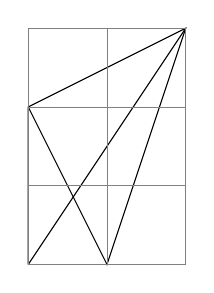
\begin{tikzpicture}
	\draw (0,0) -- (0,2) -- (2,3) -- (1,0) -- (0, 2);
	\draw (0,0) -- (2,3);
	\draw[help lines] (0, 0) grid (2, 3);
\end{tikzpicture}
\begin{lstlisting}
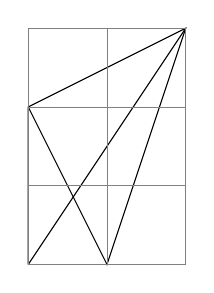
\begin{tikzpicture}
	\draw (0,0) -- (0,2) -- (2,3) -- (1,0) -- (0, 2);
	\draw (0,0) -- (2,3);
	\draw[help lines] (0, 0) grid (2, 3);
\end{tikzpicture}
\end{lstlisting}

\section{Scaling pictures} % (fold)
\label{sec:scaling_pictures}

% section scaling_pictures (end)
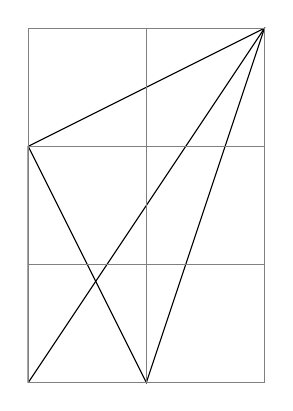
\begin{tikzpicture}[scale = 1.5]
	\draw (0,0) -- (0,2) -- (2,3) -- (1,0) -- (0, 2);
	\draw (0,0) -- (2,3);
	\draw[help lines] (0, 0) grid (2, 3);
\end{tikzpicture}
\begin{lstlisting}
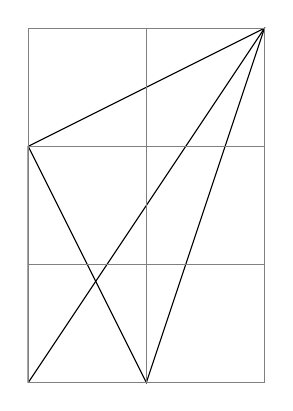
\begin{tikzpicture}[scale = 1.5]
	\draw (0,0) -- (0,2) -- (2,3) -- (1,0) -- (0, 2);
	\draw (0,0) -- (2,3);
	\draw[help lines] (0, 0) grid (2, 3);
\end{tikzpicture}
\end{lstlisting}

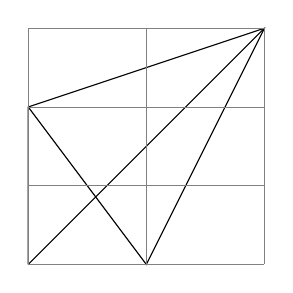
\begin{tikzpicture}[xscale = 1.5]
	\draw (0,0) -- (0,2) -- (2,3) -- (1,0) -- (0, 2);
	\draw (0,0) -- (2,3);
	\draw[help lines] (0, 0) grid (2, 3);
\end{tikzpicture}
\begin{lstlisting}
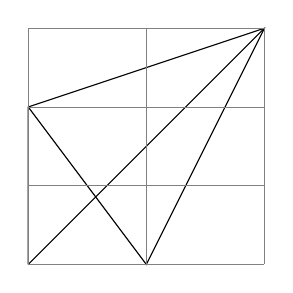
\begin{tikzpicture}[xscale = 1.5]
	\draw (0,0) -- (0,2) -- (2,3) -- (1,0) -- (0, 2);
	\draw (0,0) -- (2,3);
	\draw[help lines] (0, 0) grid (2, 3);
\end{tikzpicture}
\end{lstlisting}

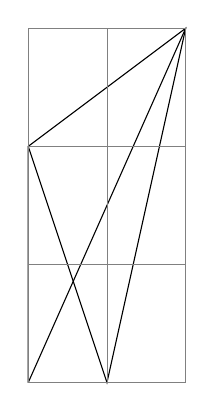
\begin{tikzpicture}[yscale = 1.5]
	\draw (0,0) -- (0,2) -- (2,3) -- (1,0) -- (0, 2);
	\draw (0,0) -- (2,3);
	\draw[help lines] (0, 0) grid (2, 3);
\end{tikzpicture}
\begin{lstlisting}
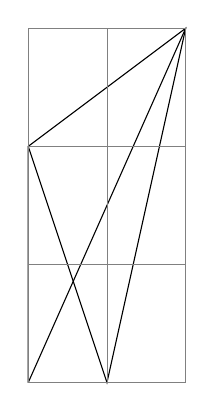
\begin{tikzpicture}[yscale = 1.5]
	\draw (0,0) -- (0,2) -- (2,3) -- (1,0) -- (0, 2);
	\draw (0,0) -- (2,3);
	\draw[help lines] (0, 0) grid (2, 3);
\end{tikzpicture}
\end{lstlisting}

\section{Arrows} % (fold)
\label{sec:arrows}
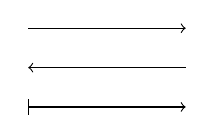
\begin{tikzpicture}
\draw [->] (0,0) -- (2, 0);
\draw [<-] (0, -0.5) -- (2,-0.5);
\draw [|->] (0,-1) -- (2,-1);
\end{tikzpicture}
\begin{lstlisting}
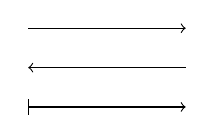
\begin{tikzpicture}
\draw [->] (0,0) -- (2, 0);
\draw [<-] (0, -0.5) -- (2,-0.5);
\draw [|->] (0,-1) -- (2,-1);
\end{tikzpicture}
\end{lstlisting}

\begin{tikzpicture}
\draw [<->] (2, 0) -- (0,0) -- (0,2);
\end{tikzpicture}
\begin{lstlisting}
\begin{tikzpicture}
\draw [<->] (2, 0) -- (0,0) -- (0,2);
\end{tikzpicture}
\end{lstlisting}

\section{Changing thickness} % (fold)
\label{sec:changing_thickness}

\begin{tikzpicture}
\draw [ultra thick] (0,1) -- (2, 1);
\draw [thick] (0,0.5) -- (2,0.5);
\draw [thin] (0,0) -- (2,0);
\draw [ultra thin] (0, -0.5) -- (2, -0.5);
\end{tikzpicture}
\begin{lstlisting}

\begin{tikzpicture}
\draw [ultra thick] (0,1) -- (2, 1);
\draw [thick] (0,0.5) -- (2,0.5);
\draw [thin] (0,0) -- (2,0);
\draw [ultra thin] (0, -0.5) -- (2, -0.5);
\end{tikzpicture}
\end{lstlisting}
Full options include 
ultra thin, very thin, thin, semithick, thick, very
thick, and ultra. Custom widths can also be used.

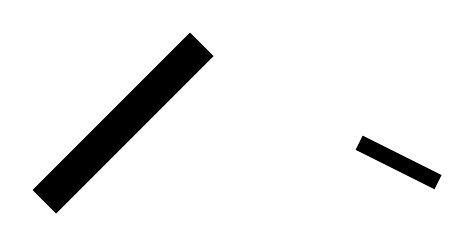
\begin{tikzpicture}
\draw [line width = 12] (0, 0) -- (2,2);
\draw [line width = 0.2 cm] (4, 0.75) -- (5, 0.25);
\end{tikzpicture}
\begin{lstlisting}
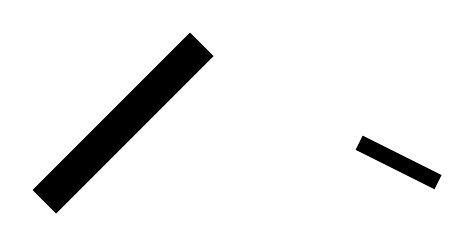
\begin{tikzpicture}
\draw [line width = 12] (0, 0) -- (2,2);
\draw [line width = 0.2 cm] (4, 0.75) -- (5, 0.25);
\end{tikzpicture}
\end{lstlisting}

\section{Dashes and dots} % (fold)
\label{sec:dashes_and_dots}
\begin{tikzpicture}
\draw [dashed, ultra thick] (0,1) -- (2,1);
\draw [dashed] (0,0.5) -- (2,0.5);
\draw [dotted] (0,0) -- (2,0);
\end{tikzpicture}
\begin{lstlisting}
\begin{tikzpicture}
\draw [dashed, ultra thick] (0,1) -- (2,1);
\draw [dashed] (0,0.5) -- (2,0.5);
\draw [dotted] (0,0) -- (2,0);
\end{tikzpicture}
\end{lstlisting}

\section{Colors} % (fold)
\label{sec:colors}
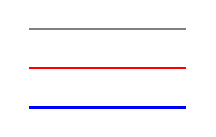
\begin{tikzpicture}
\draw [gray, thick] (0,1) -- (2, 1);
\draw [red, thick] (0,0.5) -- (2, 0.5);
\draw [blue, thick] (0,0) -- (2, 0);
\end{tikzpicture}
\begin{lstlisting}
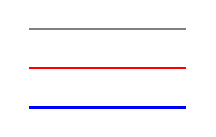
\begin{tikzpicture}
\draw [gray, thick] (0,1) -- (2, 1);
\draw [red, thick] (0,0.5) -- (2, 0.5);
\draw [blue, thick] (0,0) -- (2, 0);
\end{tikzpicture}
\end{lstlisting}
Other colors include red \tikz{\draw [red, line width = 6] (0,0) -- (0.5, 0);}
green \tikz{\draw [green, line width = 6] (0,0) -- (0.5, 0);}
yellow \tikz{\draw [yellow, line width = 6] (0,0) -- (0.5, 0);}
blue \tikz{\draw [blue, line width = 6] (0,0) -- (0.5, 0);}
cyan \tikz{\draw [cyan, line width = 6] (0,0) -- (0.5, 0);}
magenta \tikz{\draw [magenta, line width = 6] (0,0) -- (0.5, 0);}
black \tikz{\draw [black, line width = 6] (0,0) -- (0.5, 0);}
gray \tikz{\draw [gray, line width = 6] (0,0) -- (0.5, 0);}
darkgray \tikz{\draw [darkgray, line width = 6] (0,0) -- (0.5, 0);}
lightgray \tikz{\draw [lightgray, line width = 6] (0,0) -- (0.5, 0);}
brown \tikz{\draw [brown, line width = 6] (0,0) -- (0.5, 0);}
lime \tikz{\draw [lime, line width = 6] (0,0) -- (0.5, 0);}
olive \tikz{\draw [olive, line width = 6] (0,0) -- (0.5, 0);}
orange \tikz{\draw [orange, line width = 6] (0,0) -- (0.5, 0);}
pink \tikz{\draw [pink, line width = 6] (0,0) -- (0.5, 0);}
purple \tikz{\draw [purple, line width = 6] (0,0) -- (0.5, 0);}
teal \tikz{\draw [teal, line width = 6] (0,0) -- (0.5, 0);}
violet \tikz{\draw [violet, line width = 6] (0,0) -- (0.5, 0);}
white \tikz{\draw [white, line width = 6] (0,0) -- (0.5, 0);}
\begin{lstlisting}
\tikz{\draw [<color>, line width = 6] (0,0) -- (0.5, 0);}
\end{lstlisting}

\section{Curves} % (fold)
\label{sec:curves}
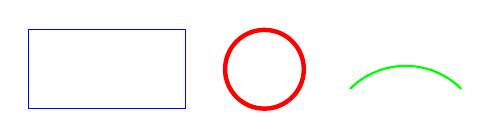
\begin{tikzpicture}
\draw [blue] (0,0) rectangle (2,1);
\draw [red, ultra thick] (3, 0.5) circle [radius = 0.5];
\draw [green, thick] (5.5,0.25) arc [radius = 1, start angle = 45, end angle = 135];
\end{tikzpicture}
\begin{lstlisting}
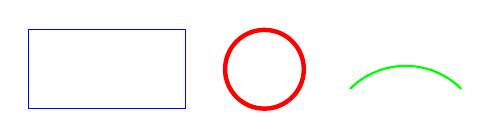
\begin{tikzpicture}
\draw [blue] (0,0) rectangle (2,1);
\draw [red, ultra thick] (3, 0.5) circle [radius = 0.5];
\draw [green, thick] (5.5,0.25) arc [radius = 1, start angle = 45, end angle = 135];
\end{tikzpicture}
\end{lstlisting}
Arc of radius 1 starts at the point (6,0), leaves it at an angle of 45 degrees and stops when its slope is 135 degrees.
To make paths take smoother turns,

\vspace{1em}
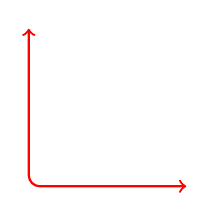
\begin{tikzpicture}
\draw [<->, rounded corners, thick, red] (0,2) -- (0,0) -- (2,0);
\end{tikzpicture}
\begin{lstlisting}
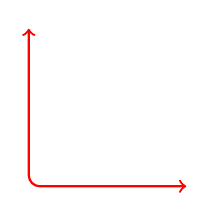
\begin{tikzpicture}
\draw [<->, rounded corners, thick, red] (0,2) -- (0,0) -- (2,0);
\end{tikzpicture}
\end{lstlisting}
Lots of anchor points can be specified explicitly to make a smoother curve.

\vspace{1em}
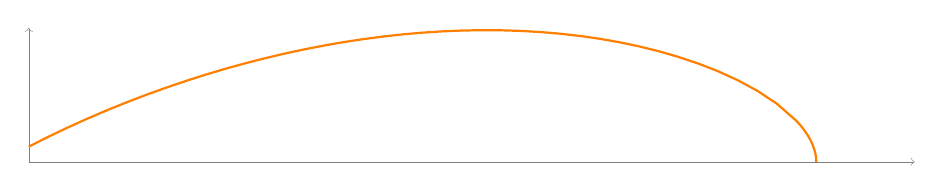
\begin{tikzpicture}[xscale=25,yscale=5]
\draw [<->, help lines] (0.6,1.34) -- (0.6,1) -- (1.05,1);
\draw[orange, thick] (0.6, 1.0385) --
(0.61, 1.06372) -- (0.62, 1.08756) -- (0.63, 1.11012) -- 
(0.64,1.13147) -- (0.65, 1.15166) -- (0.66, 1.17074) -- 
(0.67, 1.18874) -- (0.68,1.20568) -- (0.69, 1.22157) -- 
(0.7, 1.23643) -- (0.71, 1.25026) -- (0.72,1.26307) -- 
(0.73, 1.27486) -- (0.74, 1.28561) -- (0.75, 1.29534) -- 
(0.76,1.30402) -- (0.77, 1.31165) -- (0.78, 1.31821) -- 
(0.79, 1.32369) -- (0.8,1.32806) -- (0.81, 1.33131) -- 
(0.82, 1.3334) -- (0.83, 1.33431) -- (0.84,1.334) -- 
(0.85, 1.33244) -- (0.86, 1.32956) -- (0.87, 1.32533) -- 
(0.88,1.31966) -- (0.89, 1.3125) -- (0.9, 1.30373) -- 
(0.91, 1.29325) -- (0.92,1.2809) -- (0.93, 1.26649) -- 
(0.94, 1.24976) -- (0.95, 1.23032) -- (0.96,1.2076) -- 
(0.97, 1.18065) -- (0.98, 1.14763) -- (0.99, 1.1038) -- 
(0.991,1.09836) -- (0.992, 1.09261) -- (0.993, 1.0865) -- 
(0.994, 1.07994) -- (0.995,1.07282) -- (0.996, 1.06497) -- 
(0.997, 1.0561) -- (0.998, 1.04563) -- (0.999,1.03209) -- 
(0.9991, 1.03042) -- (0.9992, 1.02866) -- (0.9993,1.02679) -- 
(0.9994, 1.02478) -- (0.9995, 1.0226) -- (0.9996, 1.02019) -- 
(0.9997,1.01747) -- (0.9998, 1.01424) -- (0.9999, 1.01005) -- 
(0.9999,1.01005) -- (0.99991, 1.00953) -- (0.99992, 1.00898) -- 
(0.99993,1.0084) -- (0.99994, 1.00778) -- (0.99995, 1.0071) -- 
(0.99996,1.00634) -- (0.99997, 1.00549) -- (0.99998, 1.00448) -- 
(0.99999, 1.00317) -- (1,1) ;
\end{tikzpicture}
\begin{lstlisting}
\begin{tikzpicture}[xscale=25,yscale=5]
\draw [<->, help lines] (0.6,1.34) -- (0.6,1) -- (1.05,1);
\draw[orange, thick] (0.6, 1.0385) --
(0.61, 1.06372) -- (0.62, 1.08756) -- (0.63, 1.11012) -- 
(0.64,1.13147) -- (0.65, 1.15166) -- (0.66, 1.17074) -- 
(0.67, 1.18874) -- (0.68,1.20568) -- (0.69, 1.22157) -- 
[... lots of points ...]
(0.9991, 1.03042) -- (0.9992, 1.02866) -- (0.9993,1.02679) -- 
(0.9994, 1.02478) -- (0.9995, 1.0226) -- (0.9996, 1.02019) -- 
(0.9997,1.01747) -- (0.9998, 1.01424) -- (0.9999, 1.01005) -- 
(0.9999,1.01005) -- (0.99991, 1.00953) -- (0.99992, 1.00898) -- 
(0.99993,1.0084) -- (0.99994, 1.00778) -- (0.99995, 1.0071) -- 
(0.99996,1.00634) -- (0.99997, 1.00549) -- (0.99998, 1.00448) -- 
(0.99999, 1.00317) -- (1,1) ;
\end{tikzpicture}
\end{lstlisting}
A simpler way to draw a curve is to specify the inlet and exit points, and the inlet and exit angles. 

\noindent
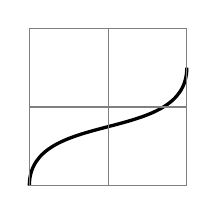
\begin{tikzpicture}
\draw[very thick] (0,0) to [out=90,in=-90] (2,1.5);
\draw[gray] (0,0) grid (2,2);
\end{tikzpicture}
\begin{lstlisting}
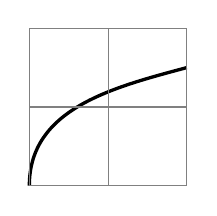
\begin{tikzpicture}
\draw[very thick] (0,0) to [out=90,in=195] (2,1.5);
\draw[gray] (0,0) grid (2,2);
\end{tikzpicture}
\end{lstlisting}
To decipher the angles, 
\begin{itemize}
	\item Draw a vector at the beginning, (0,0) pointing \emph{right} along the base of the figure. Rotate the vector \emph{counterclockwise} until it is tangent with the drawn curve. The angle turned is the \texttt{\small{out}} angle.
	\item Draw a vector at the end, (2, 1.5) pointing to the \emph{left} parallel to the base of the figure. Rotate the vector \emph{counterclockwise} until it is tangent with the drawn curve. The angle turned is the \texttt{\small{in}} angle. \end{itemize}

\noindent
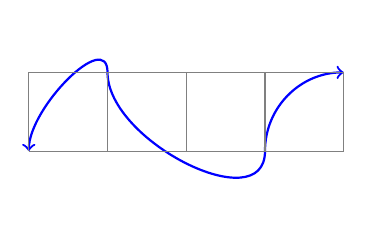
\begin{tikzpicture}
\draw [<->, thick, blue] (0,0) to [out = 90, in = 90] (1,1) [out = -90, in = -90] to (3,0) to [out = 90, in = 180] (4,1);
\draw [gray] (0,0) grid (4,1);
\end{tikzpicture}
\begin{lstlisting}
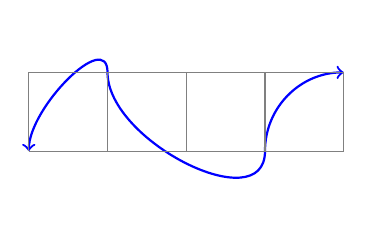
\begin{tikzpicture}
\draw [<->, thick, blue] (0,0) to [out = 90, in = 90] (1,1) [out = -90, in = -90] to (3,0) to [out = 90, in = 180] (4,1);
\draw [gray] (0,0) grid (4,1);
\end{tikzpicture}
\end{lstlisting}

\section{PLotting functions} % (fold)
\label{sec:plotting_functions}
Ti\emph{k}z has a math engine to plot functions.

\vspace{1em}
\noindent
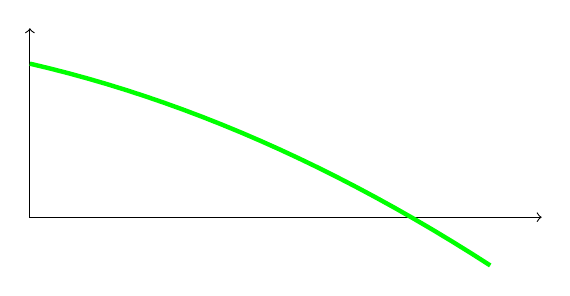
\begin{tikzpicture}[xscale = 13, yscale = 3]
\draw [<->] (0, 0.8) -- (0,0) -- (0.5, 0);
\draw [green, ultra thick, domain = 0:0.45] plot (\x, {0.65 - \x - 2*\x*\x});
\end{tikzpicture}
\begin{lstlisting}
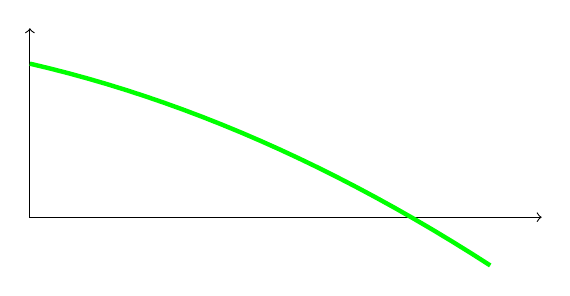
\begin{tikzpicture}[xscale = 13, yscale = 3]
\draw [<->] (0, 0.8) -- (0,0) -- (0.5, 0);
\draw [green, ultra thick, domain = 0:0.45] 
plot (\x, {0.65 - \x - 2*\x*\x});
\end{tikzpicture}
\end{lstlisting}
Available functions include {\small \texttt{factorial(\textbackslash x)}, \texttt{sqrt(\textbackslash x)}, \texttt{pow(\textbackslash x,y)}} ($x^y$){\small, \texttt{exp(\textbackslash x)}, \texttt{ln(\textbackslash x)}, \texttt{log10(\textbackslash x)}, \texttt{log2(\textbackslash x)}, \texttt{abs(\textbackslash x)}, \texttt{mod(\textbackslash x,y)}, \texttt{round(\textbackslash x)}, \texttt{floor(\textbackslash x)}, \texttt{ceil(\textbackslash x)}, \texttt{sin(\textbackslash x)}, (\texttt{sin(\textbackslash x r)}} for radians{\small ), \texttt{cos(\textbackslash x)}, \texttt{cos(\textbackslash x r)}, \texttt{tan(\textbackslash x)}, \texttt{tan(\textbackslash x r)}, \texttt{min(\textbackslash x, y)}, \texttt{max(\textbackslash x, y)}. \par} These functions can be mixed together, along with two provided constants, \texttt{e} =  2.718281828, and \texttt{pi} = 3.141592654.

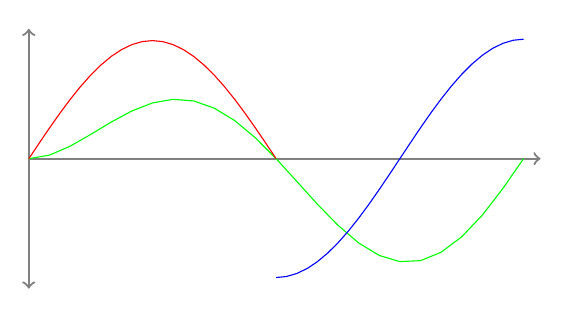
\begin{tikzpicture}[yscale=1.5]
\draw [gray, thick, ->] (0,0) -- (6.5,0);
\draw [gray, thick, <->] (0,-1.1) -- (0,1.1);
\draw [green,domain=0:2*pi] plot (\x, {(sin(\x r)* ln(\x+1))/2});
\draw [red,domain=0:pi] plot (\x, {sin(\x r)});
\draw [blue, domain=pi:2*pi] plot (\x, {cos(\x r)*exp(\x/exp(2*pi))});
\end{tikzpicture}
\begin{lstlisting}
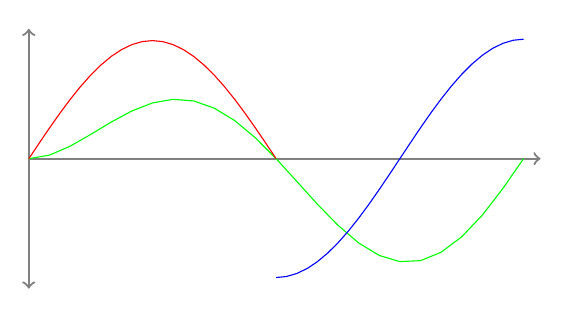
\begin{tikzpicture}[yscale=1.5]
\draw [gray, thick, ->] (0,0) -- (6.5,0);
\draw [gray, thick, <->] (0,-1.1) -- (0,1.1);
\draw [green,domain=0:2*pi] plot (\x, {(sin(\x r)* ln(\x+1))/2});
\draw [red,domain=0:pi] plot (\x, {sin(\x r)});
\draw [blue, domain=pi:2*pi] 
plot (\x, {cos(\x r)*exp(\x/exp(2*pi))});
\end{tikzpicture}
\end{lstlisting}

\section{Filling areas} % (fold)
\label{sec:filling_areas}
Closed paths can be filled.

% \begin{tikzpicture}
% \draw [fill=red,ultra thick] (0,0) rectangle (1,1);
% \draw [fill=red,ultra thick,red] (2,0) rectangle (3,1);
% \draw [blue, fill=blue] (4,0) -- (5,1) -- (4.75,0.15) -- (4,0);
% \draw [fill] (7,0.5) circle [radius=0.1];
% \draw [fill=orange] (9,0) rectangle (11,1);
% \draw [fill=white] (9.25,0.25) rectangle (10,1.5);
% \end{tikzpicture}

\noindent
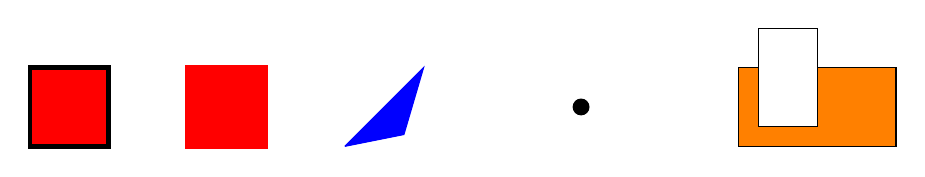
\begin{tikzpicture}
\draw [fill = red, ultra thick] (0,0) rectangle (1,1);
\draw [fill = red, ultra thick, red] (2,0) rectangle (3,1);
\draw [blue, fill = blue] (4,0) -- (5,1) -- (4.75, 0.15) -- (4,0);
\draw [fill] (7, 0.5) circle [radius = 0.1];
\draw [fill = orange] (9,0) rectangle (11,1);
\draw [fill = white] (9.25, 0.25) rectangle (10, 1.5);
\end{tikzpicture}
\begin{lstlisting}
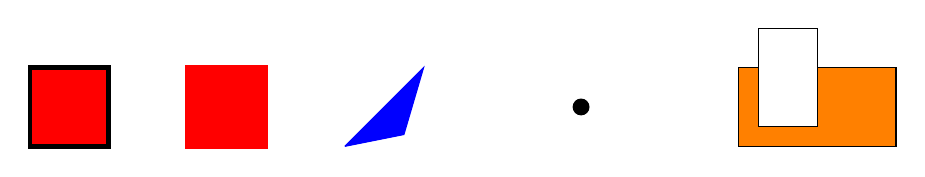
\begin{tikzpicture}
\draw [fill = red, ultra thick] (0,0) rectangle (1,1);
\draw [fill = red, ultra thick, red] (2,0) rectangle (3,1);
\draw [blue, fill = blue] (4,0) -- (5,1) -- (4.75, 0.15) -- (4,0);
\draw [fill] (7, 0.5) circle [radius = 0.1];
\draw [fill = orange] (9,0) rectangle (11,1);
\draw [fill = white] (9.25, 0.25) rectangle (10, 1.5);
\end{tikzpicture}

\end{lstlisting}
\end{document}

